%TITULO------------------------------------------------------------------------

%==============================================================================
\chapter{Modelagem de Conversores Conectados à Rede Elétrica via Filtro LCL}
\label{modelagem}
%==============================================================================

	%intro temporária, melhorar
	Este capítulo apresenta a modelagem de conversores de potência conectados à rede
    elétrica via filtro LCL. São apresentados modelos dinâmicos e em espaço de
    estados, bem como em coordenadas $\alpha \beta 0$ \cite{ref:JORGE} e em
    função de transferência, considerando a corrente $i_C$ e a tensão $v_C$
    do capacitor como variável intermediária. Modelos em tempo discreto são
    desenvolvidos, levando em conta o impacto do atraso de transporte da
    implementação digital.


\section{Modelo em Espaço de Estados - Coordenadas \emph{abc}}

    Considere um conversor trifásico conectado à rede elétrica via filtro LCL
    conforme a Fig.~\ref{fig:LCL_topologia_2}. Considere ainda a rede elétrica
    como sendo uma fonte de tensão trifásica alternada equilibrada com uma
    impedância série equivalente com característica indutiva.

    \begin{figure}[htb]
        \centering{
            %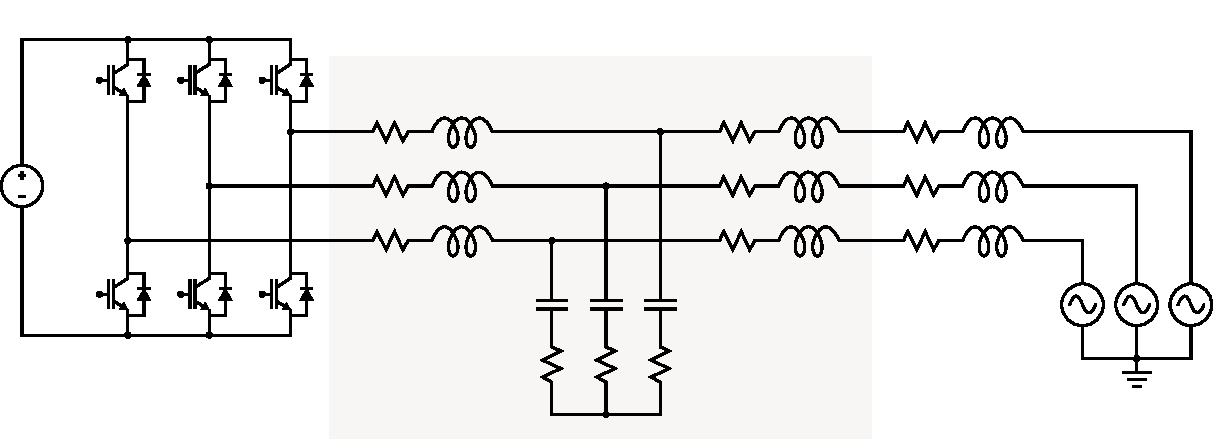
\includegraphics[width=0.9\textwidth]{img/topologia}}
            \def\svgwidth{\textwidth}
            \input{./img/topologia.pdf_tex}}
        \renewcommand\figurename{Fig.}
        \caption{Topologia do filtro LCL.}
        \label{fig:LCL_topologia_2}
    \end{figure}

    A partir das leis de Kirchhoff pode-se obter:
    %
    \begin{equation}
        u_{ab}(t) = R_1 i_{a1}(t) + L_1 \frac{d}{dt} i_{a1}(t) + v_{an}(t)
            - v_{bn}(t) - L_1 \frac{d}{dt} i_{b1}(t) - R_1 i_{b1}(t) \text{,}
    \end{equation}
    %
    \begin{equation}
        u_{bc}(t) = R_1 i_{b1}(t) + L_1 \frac{d}{dt} i_{b1}(t) + v_{bn}(t)
            - v_{cn}(t) - L_1 \frac{d}{dt} i_{c1}(t) - R_1 i_{c1}(t) \text{,}
    \end{equation}
    %
    \begin{equation}
        i_{a1}(t) + i_{b1}(t) + i_{c1}(t) = 0 \implies \frac{d}{dt} i_{a1}(t)
            + \frac{d}{dt} i_{b1}(t) + \frac{d}{dt} i_{c1}(t) = 0 \text{.}
    \end{equation}

    Além disso, das tensões nos capacitores:
    %
    \begin{equation}
        C \frac{d}{dt} v_{an}(t) = i_{a1}(t) - i_{a2}(t) \text{,}
    \end{equation}
    %
    \begin{equation}
        C \frac{d}{dt} v_{bn}(t) = i_{b1}(t) - i_{b2}(t) \text{,}
    \end{equation}
    %
    \begin{equation}
        C \frac{d}{dt} v_{an}(t) + C \frac{d}{dt} v_{bn}(t) +
            C \frac{d}{dt} v_{cn}(t) = 0 \text{.}
    \end{equation}

    E das correntes do lado da rede:
    %
    \begin{equation}
        v_{ab}(t) = R_2 i_{a2}(t) + L_2 \frac{d}{dt} i_{a2}(t) + v_a(t) - v_b(t)
            - L_2 \frac{d}{dt} i_{b2}(t) - R_2 i_{b2}(t) \text{,}
    \end{equation}
    %
    \begin{equation}
        v_{bc}(t) = R_2 i_{b2}(t) + L_2 \frac{d}{dt} i_{b2}(t) + v_b(t) - v_c(t)
            - L_2 \frac{d}{dt} i_{c2}(t) - R_2 i_{c2}(t) \text{,}
    \end{equation}
    %
    \begin{equation}
        i_{a2}(t) + i_{b2}(t) + i_{c2}(t) = 0 \implies \frac{d}{dt} i_{a2}(t) +
            \frac{d}{dt} i_{b2}(t) + \frac{d}{dt} i_{c2}(t) = 0 \text{.}
    \end{equation}

    É possível escrever esse modelo em forma matricial,
    %
    \begin{equation}
        \begin{split}
            \mathbf{L} \frac{d}{dt} \mathbf{x}_{abc}(t) & = \mathbf{Ax}_{abc}(t) +
                \mathbf{Bu}_{Labc}(t) + \mathbf{Fv}_{abc}(t) \\
            \mathbf{y}(t) & = \mathbf{C}_{abc} \mathbf{x}_{abc}(t) \text{,}
        \end{split}
    \end{equation}
    %
    na qual as variáveis de saída podem ser tanto as correntes do lado do conversor
    quanto as correntes do lado da rede. A escolha é feita através da matriz
    $\mathbf{C}_{abc}$. $\mathbf{x}_{abc}(t)$ representa os estados em coordenadas
    \emph{abc}, $\mathbf{u}_{Labc}(t)$ representa as tensões de linha aplicadas pelo
    conversor e $\mathbf{v}_{abc}(t)$ representa as tensões de fase da rede.

    Pode-se simplificar o modelo multiplicando por $\mathbf{L}^{-1}$ dos dois
    lados da igualdade, obtendo
    %
    \begin{equation}
        \begin{split}
            \frac{d}{dt} \mathbf{x}_{abc}(t) & = \mathbf{A}_{abc} \mathbf{x}_{abc}(t) +
                \mathbf{Bu}_{Labc}(t) + \mathbf{F}_{abc} \mathbf{v}_{abc}(t) \\
            \mathbf{y}(t) & = \mathbf{C}_{abc} \mathbf{x}_{abc}(t) \text{.}
        \end{split}
    \end{equation}

    É necessário representar o vetor de tensões do conversor $\mathbf{u}_{Labc}(t)$ em
    grandezas de fase, o que implica na transformação
    %
    \begin{equation}
        \mathbf{u}_{Labc}(t) = \left[
            \begin{array}{ccc}
                1 &           -1 & \phantom{-}0 \\[0.3em]
                0 & \phantom{-}1 &           -1 \\[0.3em]
                1 & \phantom{-}1 & \phantom{-}1
            \end{array}
        \right] \mathbf{u}_{abc}(t) = \mathbf{T}_{FL} \mathbf{u}_{abc}(t)
    \end{equation}

    Dessa forma, obtem-se
    %
    \begin{equation}
        \begin{split}
            \frac{d}{dt} \mathbf{x}_{abc}(t) & = \mathbf{A}_{abc} \mathbf{x}_{abc}(t) +
                \mathbf{BT}_{FL} \mathbf{u}_{abc}(t) + \mathbf{F}_{abc} \mathbf{v}_{abc}(t) \\
            \mathbf{y}(t) & = \mathbf{C}_{abc} \mathbf{x}_{abc}(t) \text{,}
        \end{split}
    \end{equation}
    %
    que é equivalente a
    %
    \begin{equation}
        \begin{split}
            \frac{d}{dt} \mathbf{x}_{abc}(t) & = \mathbf{A}_{abc} \mathbf{x}_{abc}(t) +
                \mathbf{B}_{abc} \mathbf{u}_{abc}(t) + \mathbf{F}_{abc} \mathbf{v}_{abc}(t) \\
            \mathbf{y}(t) & = \mathbf{C}_{abc} \mathbf{x}_{abc}(t) \text{.}
        \end{split}
        \label{eq:LCL_abc_espaco_estados}
    \end{equation}

    O modelo (\ref{eq:LCL_abc_espaco_estados}) apresenta acoplamento entre as variáveis
    de cada fase, o que dificulda a sua utilização em sistemas de controle. Devido à
    isso, uma transformação para desacoplamento é apresentada na seção seguinte.

\section{Modelo em Espaço de Estados - Coordenadas $\alpha \beta 0$}

    A representação de sistemas elétricos trifásicos é objeto de estudos desde o
    início de sua utilização, no começo do século XX. Dentre as primeiras contribuições
    neste sentido, encontra-se o trabalho de Charles L. Fortescue~\cite{ref:FORTESCUE},
    conhecido como a teoria de componentes simétricas, que representa um sistema trifásico
    desequilibrado em termos de três sistemas trifásicos equilibrados, chamados circuitos
    de sequência positiva, negativa e zero. Uma outra contribuição foi feita por Edith
    Clarke, com a transformação nomeada em sua homenagem~\cite{ref:CLARKE}. A transformação
    de Clarke, ou transformação $\alpha \beta 0$ permite representar um sistema trifásico
    acoplado em termos de componentes monofásicas desacopladas. Essa transformação é muito
    útil em aplicações de conversores estáticos trifásicos, visto que possibilita a
    simplificação dos modelos e do projeto dos controladores.

    A transformação $\alpha \beta 0$ é linear e invariante no tempo, e é dada por
    %
    %usando array e phantom{-} pelo alinhamento
    \begin{equation}
        \mathbf{T}_{\alpha \beta 0} = \frac{2}{3} \left[
        \begin{array}{ccc}
            1 & -\frac{1}{2} & -\frac{1}{2} \\[0.3em]
            0 & \phantom{-}\frac{\sqrt{3}}{2} & -\frac{\sqrt{3}}{2} \\[0.3em]
            \frac{1}{2} &  \phantom{-}\frac{1}{2} & \phantom{-}\frac{1}{2}
        \end{array}
        \right] \text{.}
        \label{eq:alpha_beta_0}
    \end{equation}

    Utilizando essa transformação, qualquer parâmetro em coordenadas $abc$ pode ser
    transcrito em coordenadas $\alpha \beta 0$, e vice versa
    %
    \begin{equation}
        \mathbf{T}_{\alpha \beta 0} \mathbf{x}_{abc} = \mathbf{x}_{\alpha \beta 0}
        \iff
        \mathbf{T}_{\alpha \beta 0}^{-1} \mathbf{x}_{\alpha \beta 0} = \mathbf{x}_{abc}
        \text{.}
    \end{equation}

    No projeto de controladores para sistemas elétricos trifásicos, é usual levar em
    consideração essa transformação e modelar o sistema para o caso monofásico, projetando
    o controlador considerando os equivalentes nas coordenadas $\alpha$ e $\beta$. A
    Fig~\ref{fig:LCL_geral} apresenta a estrutura do sistema para o caso monofásico. Neste
    caso, as indutâncias do filtro são: $L_1$ do lado do conversor e $L_2$ do lado da rede,
    $C$ é a capacitância do filtro e $L_g$ é a indutância da rede elétrica. A tensão gerada
    pelo conversor é representada por $u_{\alpha}$ e a rede elétrica é representada por
    $v_{\alpha}$.

    \begin{figure}[htb]
        \centering{
            %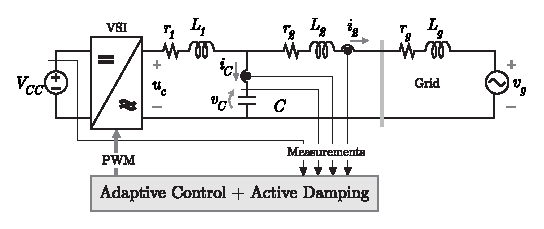
\includegraphics[width=0.9\textwidth]{img/LCL_geral}}
            \def\svgwidth{\textwidth}
            \input{./img/LCL_geral.pdf_tex}}
        \renewcommand\figurename{Fig.}
        \caption{Filtro LCL para o caso monofásico.}
        \label{fig:LCL_geral}
    \end{figure}

    Visto que a transformação (\ref{eq:alpha_beta_0}) é invariante no tempo, ela pode ser
    aplicada ao modelo (\ref{eq:LCL_abc_espaco_estados}). Dessa forma, tem-se que
    %
    \begin{equation}
        \begin{split}
            \mathbf{T}_{\alpha \beta 0} \frac{d}{dt} \mathbf{x}_{abc}(t) & =
                \mathbf{T}_{\alpha \beta 0} \mathbf{A}_{abc} \mathbf{x}_{abc}(t) +
                \mathbf{T}_{\alpha \beta 0} \mathbf{B}_{abc} \mathbf{u}_{abc}(t) +
                \mathbf{T}_{\alpha \beta 0} \mathbf{F}_{abc} \mathbf{v}_{abc}(t) \\
            \mathbf{T}_{\alpha \beta 0} \mathbf{y}_{abc}(t) & = \mathbf{T}_{\alpha \beta 0}
                \mathbf{C}_{abc} \mathbf{x}_{abc}(t) \text{,}
        \end{split}
    \end{equation}
    %
    isto é,
    %
    \begin{equation}
        \begin{split}
            \frac{d}{dt} \mathbf{x}_{\alpha \beta 0}(t) & =
                \mathbf{A}_{\alpha \beta 0} \mathbf{x}_{\alpha \beta 0}(t) +
                \mathbf{B}_{\alpha \beta 0} \mathbf{u}_{\alpha \beta 0}(t) +
                \mathbf{F}_{\alpha \beta 0} \mathbf{v}_{\alpha \beta 0}(t) \\
            \mathbf{y}_{\alpha \beta 0}(t) & = \mathbf{C}_{\alpha \beta 0}
                \mathbf{x}_{\alpha \beta 0}(t) \text{.}
        \end{split}
        \label{eq:LCL_ab0_espaco_estados}
    \end{equation}

    O modelo (\ref{eq:LCL_ab0_espaco_estados}) representa o sistema na forma de dois
    sistemas monofásicos desacoplados associados ao eixo $\alpha$ e ao eixo $\beta$. O
    eixo $0$ pode ser desconsiderado, já que não há caminho para circulação de corrente
    de sequência zero.

\section{Modelo em Função de Transferência}

    Uma forma conveniente de modelar o sistema é através de impedâncias
    complexas~\cite{ref:XU}. As indutâncias e a capacitância do filtro podem ser
    representadas pelas seguintes impedâncias
    %
    \begin{equation}
        \begin{split}
            Z_i & = r_1 + L_1 s \text{,} \\
            Z_C & = \frac{1}{s C} \text{,} \\
            Z_g & = r_2 + r_g + \left( L_2 + L_g \right) s \text{.}
        \end{split}
    \end{equation}

    A impedância do lado da rede $Z_g$ engloba duas indutâncias: uma indutância projetada,
    $L_2$, e uma indutância desconhecida que é a indutância da rede elétrica $L_g$. Escolheu-se
    essa forma de representação de modo a explicitar a incerteza paramétrica, apesar de $L_2$
    ser uma indutância projetada. Além disso, é importante esclarecer que a tensão da rede
    $v_g$ pode ser desprezada na obtenção do modelo, visto que é um distúrbio exógeno que
    deve ser rejeitado pelo controlador adaptativo.

    % A Fig.~\ref{fig:estrutura_geral_cascata} demonstra a estrutura de controle utilizada.

    % \begin{figure}[htb]
    %     \centering{
    %         %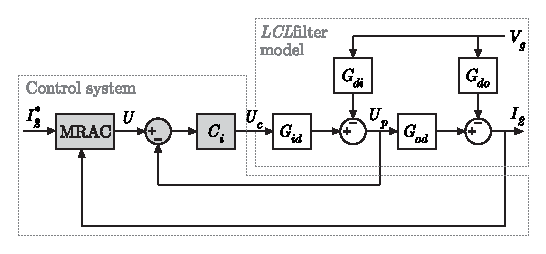
\includegraphics[width=0.9\textwidth]{img/cascade_general}}
    %         \def\svgwidth{0.9\textwidth}
    %         \input{./img/multiloop_geral.pdf_tex}}
    %     \renewcommand\figurename{Fig.}
    %     \caption{Diagrama de blocos demonstrando a estrutura geral de controle.}
    %     \label{fig:estrutura_geral_cascata}
    % \end{figure}

    % Observa-se que $U_p$ indica a variável de controle intermediária utilizada para
    % implementar a malha interna e realizar o amortecimento ativo da ressonância do filtro,
    % podendo ser $V_C$ ou $I_C$. O controlador adaptativo na malha externa gera a referência
    % $U$ para a malha interna, que por sua vez gera a ação de controle $U_c$ implementada
    % via PWM.

    Considerando a estrutura da Fig.~\ref{fig:LCL_geral} e desprezando o distúrbio da
    rede $v_g$, obtém-se as seguintes expressões a partir das leis de Kirchhoff
    %
    \begin{equation}
        \frac{V_C}{U_c} = \frac{Z_C Z_g}{Z_i \left( Z_C + Z_g \right) + Z_C Z_g}
        \text{,}
        \label{eq:vc_uc}
    \end{equation}
    %
    \begin{equation}
        \frac{I_C}{U_c} = \frac{Z_g}{Z_i \left( Z_C + Z_g \right) + Z_C Z_g}
        \text{,}
        \label{eq:ic_uc}
    \end{equation}
    %
    \begin{equation}
        \frac{I_2}{U_c} = \frac{Z_C}{Z_i \left( Z_C + Z_g \right) + Z_C Z_g}
        \text{.}
    \end{equation}

    Do ponto de vista de amortecimento ativo, todo e qualquer elemento resistivo
    que se encontre no sistema irá colaborar com o amortecimento, embora de forma
    passiva. Por esse motivo, as resistências são desprezadas na modelagem do
    sistema, visto que isto irá facilitar a modelagem e criar um caso pior do que
    o que se encontra na prática.

    A discretização destas funções de transferência é feita conforme realizado
    em \cite{ref:PARKER}, incluindo um retentor de ordem zero (ZOH) e aplicando a
    transformada $\mathcal{Z}$. Dessa forma, considerando o atraso de tempo associado
    à implementação digital, obtém-se
    %
    \begin{equation}
        G_d (z) = \frac{I_2}{U_c} = K_1 \frac{1}{z \left( z-1 \right)}
        - \frac{K_1 \sen \left( \omega_n T_s \right) }{\omega_n T_s}
        \frac{z-1}{z \left( z^2 - 2 \cos\left( \omega_n T_s \right) z +1 \right) }
        \text{,}
    \end{equation}
    %
    onde $T_s$ é o período de amostragem e
    %
    \begin{equation}
        K_1 = \frac{T_s}{L1 + L2 + Lg} \text{,}
    \end{equation}
    %
    \begin{equation}
        \omega_n = \sqrt{\frac{ L_1 + L_2 + L_g }{ L_1 C \left( L_2 + L_g \right)}}
        \text{.}
    \end{equation}

    No caso em que a variável intermediária é a tensão do capacitor $V_C$, para
    relacionar $I_2$ com $V_C$ é necessário discretizar a equação~(\ref{eq:vc_uc})
    %
    \begin{equation}
        G_{id}(z) = \frac{2 \sen^2 \left( \omega_n \frac{T_s}{2} \right)}{L_1 C \omega_n^2}
            \frac{z+1}{z \left( z^2 - \cos \left( \omega_n T_s \right) z + 1 \right)}
            \text{.}
    \end{equation}

    Dessa forma, a relação $G_{od}$ entre $I_2$ e $V_C$ é
    %
    \begin{equation}
        G_{od}(z) = \frac{I_2}{V_C} = \frac{G_d}{G_{id}} \text{.}
    \end{equation}

    De forma semelhante, no caso em que a variável intermediária é a corrente do
    capacitor $I_C$, para relacionar $I_2$ com $I_C$ é necessário discretizar a
    equação~(\ref{eq:ic_uc})
    %
    \begin{equation}
        G_{id}(z) = \frac{\sen \left( \omega_n T_s \right)}{\omega_n L_1}
            \frac{z-1}{z \left( z^2 - \cos \left( \omega_n T_s \right) z + 1 \right)}
            \text{,}
    \end{equation}
    %
    e assim
    %
    \begin{equation}
        G_{od}(z) = \frac{I_2}{I_C} = \frac{G_d}{G_{id}} \text{.}
    \end{equation}


\section{Efeitos da Discretização}

    Plantas de fase mínima, ou seja, aquelas que apresentam zeros apenas no
    semi-plano esquerdo do plano $s$, permitem que os efeitos de zeros indesejados
    sejam cancelados pela alocação de pólos do controlador. Isso é impossível,
    no entanto, no caso de plantas de fase não-mínima, visto que a alocação de
    pólos do controlador no semi-plano esquerdo resulta em instabilidade.

    Por isso, é importante observar que a discretização de um sistema pode implicar
    em problemas do ponto de vista de controle. Mesmo uma planta de fase mínima em
    tempo contínuo pode apresentar zeros de fase não-mínima após a discretização.
    De fato, de uma forma mais geral, plantas em tempo contínuo com grau relativo
    $n \ge 2$ apresentam zeros de discretização \cite{ref:ASTROM}. Esse é o caso
    do filtro LCL quando a variável controlada é a corrente do lado da rede.

    %Para fazer subreferências:
    %
    %As figuras \ref{fig:pzmap_ic_vc}.\subref{fig:pzmap_ic} e
    %\ref{fig:pzmap_ic_vc}.\subref{fig:pzmap_vc} apresentam o diagrama de pólos
    %e zeros para o filtro LCL e demonstram esse efeito.

    A figura \ref{fig:pzmap_ic_vc} apresenta o diagrama de pólos e zeros para o
    filtro LCL e demonstra esse efeito.

    \begin{figure}[htb]
        \centering
        \subfloat[Corrente do capacitor.]{\label{fig:pzmap_ic}
            {% This file was created by matlab2tikz v0.4.7 running on MATLAB 7.14.
% Copyright (c) 2008--2014, Nico Schlömer <nico.schloemer@gmail.com>
% All rights reserved.
% Minimal pgfplots version: 1.3
% 
% The latest updates can be retrieved from
%   http://www.mathworks.com/matlabcentral/fileexchange/22022-matlab2tikz
% where you can also make suggestions and rate matlab2tikz.
% 
%
% defining custom colors
\definecolor{mycolor1}{rgb}{0.66667,0.66667,0.66667}%
%
\begin{tikzpicture}

\begin{axis}[%
width=0.8\textwidth,
height=0.461611624834875\textwidth,
scale only axis,
xmin=-4,
xmax=1.2,
xtick={-4, -3, -2, -1,  0,  1},
xlabel={Eixo Real},
ymin=-1.4,
ymax=1.4,
ytick={-1,  0,  1},
ylabel={Eixo Imaginário},
axis x line*=bottom,
axis y line*=left
]
\addplot [color=mycolor1,dotted,line width=1.0pt,forget plot]
  table[row sep=crcr]{1	0\\
0.987688340595138	0.156434465040231\\
0.951056516295154	0.309016994374947\\
0.891006524188368	0.453990499739547\\
0.809016994374947	0.587785252292473\\
0.707106781186548	0.707106781186547\\
0.587785252292473	0.809016994374947\\
0.453990499739547	0.891006524188368\\
0.309016994374947	0.951056516295154\\
0.156434465040231	0.987688340595138\\
6.12323399573677e-17	1\\
-0.156434465040231	0.987688340595138\\
-0.309016994374947	0.951056516295154\\
-0.453990499739547	0.891006524188368\\
-0.587785252292473	0.809016994374947\\
-0.707106781186547	0.707106781186548\\
-0.809016994374947	0.587785252292473\\
-0.891006524188368	0.453990499739547\\
-0.951056516295154	0.309016994374948\\
-0.987688340595138	0.156434465040231\\
-1	1.22464679914735e-16\\
};
\addplot [color=mycolor1,dotted,line width=1.0pt,forget plot]
  table[row sep=crcr]{1	0\\
0.972218045703082	0.153984211042097\\
0.921496791140463	0.299412457456957\\
0.849791018366557	0.432990150609548\\
0.759508516401756	0.551815237548133\\
0.653437051516106	0.653437051516106\\
0.534664304371591	0.735902282058355\\
0.406492952796512	0.797787339572243\\
0.272353130096494	0.83821674479613\\
0.135714483753824	0.856867527364047\\
5.22899666167123e-17	0.853959960588124\\
-0.131496350792703	0.830235283991667\\
-0.255686250369537	0.786921363444393\\
-0.369756251949576	0.725687504552447\\
-0.47122811850853	0.648589862732789\\
-0.558009078759514	0.558009078759514\\
-0.628431083783263	0.456581908289041\\
-0.681278445058817	0.347128705949459\\
-0.715803538350409	0.232578668243255\\
-0.731730559897045	0.115894735197653\\
-0.729247614287671	8.9307075662324e-17\\
};
\addplot [color=mycolor1,dotted,line width=1.0pt,forget plot]
  table[row sep=crcr]{1	0\\
0.956521682769877	0.151498151383791\\
0.891982039736211	0.289822533396298\\
0.809292583610082	0.412355167436434\\
0.711634858347723	0.517032989000692\\
0.602364630186427	0.602364630186426\\
0.484917701774751	0.667431957639199\\
0.362719588349683	0.711877274647591\\
0.239101059900595	0.735877395777214\\
0.117221283062812	0.740106053489981\\
4.44354699422903e-17	0.725686295399261\\
-0.109940132237539	0.694134676438339\\
-0.210320240583588	0.647299141978847\\
-0.299240493845688	0.587292536894097\\
-0.375203754387119	0.516423664031337\\
-0.437127756959533	0.437127756959533\\
-0.484346224770267	0.351898130574443\\
-0.516599582217932	0.263220634338226\\
-0.534016141209622	0.173512362385299\\
-0.537084820159711	0.0850658786478001\\
-0.526620599330303	6.44924231334916e-17\\
};
\addplot [color=mycolor1,dotted,line width=1.0pt,forget plot]
  table[row sep=crcr]{1	0\\
0.940082788364644	0.148894486293864\\
0.86158608093073	0.279946287694513\\
0.768279786681378	0.391458103646313\\
0.663960650859636	0.482395649771645\\
0.552351927561387	0.552351927561387\\
0.437014383712816	0.601498696728173\\
0.321269860940431	0.630527604183869\\
0.208138182971344	0.640583459188477\\
0.100287778328637	0.633192112325829\\
3.73630739569174e-17	0.610185303761559\\
-0.0908532273476425	0.573624701779294\\
-0.170819110593797	0.525727164509449\\
-0.238861981883349	0.468793035010043\\
-0.294350736089166	0.40513903143051\\
-0.337037028702328	0.337037028702328\\
-0.367025664975262	0.266659754473976\\
-0.384738677688982	0.196034147687371\\
-0.390874612629551	0.127002860400749\\
-0.386364521398959	0.0611941284830315\\
-0.372326104926586	4.55967972637346e-17\\
};
\addplot [color=mycolor1,dotted,line width=1.0pt,forget plot]
  table[row sep=crcr]{1	0\\
0.922246029428501	0.146069421212559\\
0.829201462983264	0.269423887468404\\
0.725373165529273	0.369596088217499\\
0.614985835074999	0.446813363302878\\
0.501902475185001	0.501902475185001\\
0.38956496084428	0.536190168955128\\
0.280953750703967	0.551402782692681\\
0.178565395716864	0.549567778706978\\
0.0844061798404073	0.532919645815306\\
3.08495992433718e-17	0.50381218919366\\
-0.0735915548753502	0.464638791061534\\
-0.135739038566523	0.417761804348184\\
-0.186207014322272	0.365451842507638\\
-0.225110018726605	0.309837359892227\\
-0.252864584784672	0.252864584784672\\
-0.270139142845401	0.196267575756099\\
-0.277803443075876	0.141547924204336\\
-0.27687894570066	0.0899634229303457\\
-0.268491413422519	0.0425248622468694\\
-0.253826721980109	3.10848082611005e-17\\
};
\addplot [color=mycolor1,dotted,line width=1.0pt,forget plot]
  table[row sep=crcr]{1	0\\
0.902056570675584	0.142871725087523\\
0.793293726869509	0.257756756757911\\
0.678769666307395	0.345850419328459\\
0.562876391436159	0.408953636388562\\
0.449318435861499	0.449318435861499\\
0.341115747349381	0.469505547439701\\
0.24062663375655	0.472256359314945\\
0.149586755320764	0.460380694230177\\
0.069160331541479	0.436661148025441\\
2.47240337905553e-17	0.403774113610049\\
-0.057687904157153	0.364227092250654\\
-0.104075505986926	0.320311471399148\\
-0.139645446506012	0.274069620358657\\
-0.165124892040398	0.227274916024158\\
-0.18142315316863	0.18142315316863\\
-0.189574186252466	0.137733708524426\\
-0.190684892879101	0.0971588057560207\\
-0.185889806735969	0.0603992595374446\\
-0.176312467991919	0.0279251515651378\\
-0.16303353482158	1.99658496572927e-17\\
};
\addplot [color=mycolor1,dotted,line width=1.0pt,forget plot]
  table[row sep=crcr]{1	0\\
0.877921760602431	0.139049146701748\\
0.751411952540787	0.244148543365328\\
0.625732257688895	0.318826509862098\\
0.505011411193747	0.36691226736026\\
0.392341669548685	0.392341669548685\\
0.289890514921595	0.399000063654162\\
0.199020572856858	0.390599867100522\\
0.120411913496453	0.370589763847805\\
0.0541820486548744	0.34209199176291\\
1.88512313530119e-17	0.307863971328499\\
-0.042808222513439	0.270280479734772\\
-0.075164540154518	0.231332667812908\\
-0.0981551954909503	0.192640417840451\\
-0.112959067758674	0.155474818616317\\
-0.120787864504912	0.120787864504912\\
-0.122837744156894	0.0892468451742257\\
-0.120251626285951	0.0612712639357851\\
-0.114091236431876	0.0370704898842818\\
-0.105317799143806	0.0166807006736036\\
-0.0947802248421549	1.16072298975411e-17\\
};
\addplot [color=mycolor1,dotted,line width=1.0pt,forget plot]
  table[row sep=crcr]{1	0\\
0.84674396664984	0.134111069256013\\
0.698989566160914	0.227115477506975\\
0.561406498364893	0.286050898428465\\
0.437004973478602	0.317502698182059\\
0.327450698344114	0.327450698344114\\
0.233352139914598	0.321181666481713\\
0.154515499860225	0.303253743289057\\
0.0901653834921457	0.27750051639687\\
0.0391311034995635	0.247064063991275\\
1.31311479217367e-17	0.214447919692096\\
-0.0287598398096346	0.181582482159892\\
-0.0487044416812479	0.149896858349689\\
-0.0613430200940395	0.120392455675976\\
-0.06808779312177	0.0937148074575858\\
-0.0702211210616195	0.0702211210616195\\
-0.068876740220244	0.0500418809603846\\
-0.0650321343871793	0.0331355275052096\\
-0.0595094084547913	0.0193357789181307\\
-0.0529823745536039	0.00839158374073751\\
-0.0459879102602678	5.63189470997126e-18\\
};
\addplot [color=mycolor1,dotted,line width=1.0pt,forget plot]
  table[row sep=crcr]{1	0\\
0.801053465278425	0.126874404768154\\
0.625589539649299	0.203266363189334\\
0.475341369738971	0.242198525079547\\
0.350045057714404	0.254322621147605\\
0.24813777530853	0.24813777530853\\
0.167289292234614	0.230253957320141\\
0.104794333468008	0.205670459781722\\
0.0578515468028918	0.178048753195384\\
0.0237523524567972	0.149966451301199\\
7.54043881219821e-18	0.123144711070133\\
-0.0156239119173694	0.0986454975334405\\
-0.0250311775652273	0.0770380431086105\\
-0.0298254673925332	0.0585357756361869\\
-0.0313184856998208	0.0431061974937683\\
-0.0305568546459545	0.0305568546459545\\
-0.0283545570469435	0.0206007915573586\\
-0.0253272293454815	0.012904867916705\\
-0.021925762268643	0.00712411201600239\\
-0.0184675753156993	0.00292497658052826\\
-0.0151646198645466	1.85713031774033e-18\\
};
\addplot [color=mycolor1,dotted,line width=1.0pt,forget plot]
  table[row sep=crcr]{1	0\\
0.714110955679367	0.113104064044896\\
0.497161927717827	0.161537702532642\\
0.336758208677056	0.171586877647116\\
0.221075553032581	0.160620791180475\\
0.139705610200823	0.139705610200823\\
0.0839640345306934	0.115566579097864\\
0.0468885871776745	0.0920240337831981\\
0.0230753615892199	0.0710186604775083\\
0.00844586939409394	0.0533251206797082\\
2.39022368106624e-18	0.0390353150431684\\
-0.00441505277265522	0.0278755461307222\\
-0.00630567510971132	0.0194068724759343\\
-0.00669794782622876	0.0131454627690819\\
-0.0062698831862128	0.00862975386096949\\
-0.0054534525074872	0.0054534525074872\\
-0.00451117782354635	0.00327756254020109\\
-0.00359218715027031	0.00183031077240959\\
-0.00277223578568335	0.000900754009370227\\
-0.00208156288544739	0.000329687172611911\\
-0.00152375582051941	1.86606268828125e-19\\
};
\addplot [color=mycolor1,dotted,line width=1.0pt,forget plot]
  table[row sep=crcr]{1	-0\\
0.987688340595138	-0.156434465040231\\
0.951056516295154	-0.309016994374947\\
0.891006524188368	-0.453990499739547\\
0.809016994374947	-0.587785252292473\\
0.707106781186548	-0.707106781186547\\
0.587785252292473	-0.809016994374947\\
0.453990499739547	-0.891006524188368\\
0.309016994374947	-0.951056516295154\\
0.156434465040231	-0.987688340595138\\
6.12323399573677e-17	-1\\
-0.156434465040231	-0.987688340595138\\
-0.309016994374947	-0.951056516295154\\
-0.453990499739547	-0.891006524188368\\
-0.587785252292473	-0.809016994374947\\
-0.707106781186547	-0.707106781186548\\
-0.809016994374947	-0.587785252292473\\
-0.891006524188368	-0.453990499739547\\
-0.951056516295154	-0.309016994374948\\
-0.987688340595138	-0.156434465040231\\
-1	-1.22464679914735e-16\\
};
\addplot [color=mycolor1,dotted,line width=1.0pt,forget plot]
  table[row sep=crcr]{1	-0\\
0.972218045703082	-0.153984211042097\\
0.921496791140463	-0.299412457456957\\
0.849791018366557	-0.432990150609548\\
0.759508516401756	-0.551815237548133\\
0.653437051516106	-0.653437051516106\\
0.534664304371591	-0.735902282058355\\
0.406492952796512	-0.797787339572243\\
0.272353130096494	-0.83821674479613\\
0.135714483753824	-0.856867527364047\\
5.22899666167123e-17	-0.853959960588124\\
-0.131496350792703	-0.830235283991667\\
-0.255686250369537	-0.786921363444393\\
-0.369756251949576	-0.725687504552447\\
-0.47122811850853	-0.648589862732789\\
-0.558009078759514	-0.558009078759514\\
-0.628431083783263	-0.456581908289041\\
-0.681278445058817	-0.347128705949459\\
-0.715803538350409	-0.232578668243255\\
-0.731730559897045	-0.115894735197653\\
-0.729247614287671	-8.9307075662324e-17\\
};
\addplot [color=mycolor1,dotted,line width=1.0pt,forget plot]
  table[row sep=crcr]{1	-0\\
0.956521682769877	-0.151498151383791\\
0.891982039736211	-0.289822533396298\\
0.809292583610082	-0.412355167436434\\
0.711634858347723	-0.517032989000692\\
0.602364630186427	-0.602364630186426\\
0.484917701774751	-0.667431957639199\\
0.362719588349683	-0.711877274647591\\
0.239101059900595	-0.735877395777214\\
0.117221283062812	-0.740106053489981\\
4.44354699422903e-17	-0.725686295399261\\
-0.109940132237539	-0.694134676438339\\
-0.210320240583588	-0.647299141978847\\
-0.299240493845688	-0.587292536894097\\
-0.375203754387119	-0.516423664031337\\
-0.437127756959533	-0.437127756959533\\
-0.484346224770267	-0.351898130574443\\
-0.516599582217932	-0.263220634338226\\
-0.534016141209622	-0.173512362385299\\
-0.537084820159711	-0.0850658786478001\\
-0.526620599330303	-6.44924231334916e-17\\
};
\addplot [color=mycolor1,dotted,line width=1.0pt,forget plot]
  table[row sep=crcr]{1	-0\\
0.940082788364644	-0.148894486293864\\
0.86158608093073	-0.279946287694513\\
0.768279786681378	-0.391458103646313\\
0.663960650859636	-0.482395649771645\\
0.552351927561387	-0.552351927561387\\
0.437014383712816	-0.601498696728173\\
0.321269860940431	-0.630527604183869\\
0.208138182971344	-0.640583459188477\\
0.100287778328637	-0.633192112325829\\
3.73630739569174e-17	-0.610185303761559\\
-0.0908532273476425	-0.573624701779294\\
-0.170819110593797	-0.525727164509449\\
-0.238861981883349	-0.468793035010043\\
-0.294350736089166	-0.40513903143051\\
-0.337037028702328	-0.337037028702328\\
-0.367025664975262	-0.266659754473976\\
-0.384738677688982	-0.196034147687371\\
-0.390874612629551	-0.127002860400749\\
-0.386364521398959	-0.0611941284830315\\
-0.372326104926586	-4.55967972637346e-17\\
};
\addplot [color=mycolor1,dotted,line width=1.0pt,forget plot]
  table[row sep=crcr]{1	-0\\
0.922246029428501	-0.146069421212559\\
0.829201462983264	-0.269423887468404\\
0.725373165529273	-0.369596088217499\\
0.614985835074999	-0.446813363302878\\
0.501902475185001	-0.501902475185001\\
0.38956496084428	-0.536190168955128\\
0.280953750703967	-0.551402782692681\\
0.178565395716864	-0.549567778706978\\
0.0844061798404073	-0.532919645815306\\
3.08495992433718e-17	-0.50381218919366\\
-0.0735915548753502	-0.464638791061534\\
-0.135739038566523	-0.417761804348184\\
-0.186207014322272	-0.365451842507638\\
-0.225110018726605	-0.309837359892227\\
-0.252864584784672	-0.252864584784672\\
-0.270139142845401	-0.196267575756099\\
-0.277803443075876	-0.141547924204336\\
-0.27687894570066	-0.0899634229303457\\
-0.268491413422519	-0.0425248622468694\\
-0.253826721980109	-3.10848082611005e-17\\
};
\addplot [color=mycolor1,dotted,line width=1.0pt,forget plot]
  table[row sep=crcr]{1	-0\\
0.902056570675584	-0.142871725087523\\
0.793293726869509	-0.257756756757911\\
0.678769666307395	-0.345850419328459\\
0.562876391436159	-0.408953636388562\\
0.449318435861499	-0.449318435861499\\
0.341115747349381	-0.469505547439701\\
0.24062663375655	-0.472256359314945\\
0.149586755320764	-0.460380694230177\\
0.069160331541479	-0.436661148025441\\
2.47240337905553e-17	-0.403774113610049\\
-0.057687904157153	-0.364227092250654\\
-0.104075505986926	-0.320311471399148\\
-0.139645446506012	-0.274069620358657\\
-0.165124892040398	-0.227274916024158\\
-0.18142315316863	-0.18142315316863\\
-0.189574186252466	-0.137733708524426\\
-0.190684892879101	-0.0971588057560207\\
-0.185889806735969	-0.0603992595374446\\
-0.176312467991919	-0.0279251515651378\\
-0.16303353482158	-1.99658496572927e-17\\
};
\addplot [color=mycolor1,dotted,line width=1.0pt,forget plot]
  table[row sep=crcr]{1	-0\\
0.877921760602431	-0.139049146701748\\
0.751411952540787	-0.244148543365328\\
0.625732257688895	-0.318826509862098\\
0.505011411193747	-0.36691226736026\\
0.392341669548685	-0.392341669548685\\
0.289890514921595	-0.399000063654162\\
0.199020572856858	-0.390599867100522\\
0.120411913496453	-0.370589763847805\\
0.0541820486548744	-0.34209199176291\\
1.88512313530119e-17	-0.307863971328499\\
-0.042808222513439	-0.270280479734772\\
-0.075164540154518	-0.231332667812908\\
-0.0981551954909503	-0.192640417840451\\
-0.112959067758674	-0.155474818616317\\
-0.120787864504912	-0.120787864504912\\
-0.122837744156894	-0.0892468451742257\\
-0.120251626285951	-0.0612712639357851\\
-0.114091236431876	-0.0370704898842818\\
-0.105317799143806	-0.0166807006736036\\
-0.0947802248421549	-1.16072298975411e-17\\
};
\addplot [color=mycolor1,dotted,line width=1.0pt,forget plot]
  table[row sep=crcr]{1	-0\\
0.84674396664984	-0.134111069256013\\
0.698989566160914	-0.227115477506975\\
0.561406498364893	-0.286050898428465\\
0.437004973478602	-0.317502698182059\\
0.327450698344114	-0.327450698344114\\
0.233352139914598	-0.321181666481713\\
0.154515499860225	-0.303253743289057\\
0.0901653834921457	-0.27750051639687\\
0.0391311034995635	-0.247064063991275\\
1.31311479217367e-17	-0.214447919692096\\
-0.0287598398096346	-0.181582482159892\\
-0.0487044416812479	-0.149896858349689\\
-0.0613430200940395	-0.120392455675976\\
-0.06808779312177	-0.0937148074575858\\
-0.0702211210616195	-0.0702211210616195\\
-0.068876740220244	-0.0500418809603846\\
-0.0650321343871793	-0.0331355275052096\\
-0.0595094084547913	-0.0193357789181307\\
-0.0529823745536039	-0.00839158374073751\\
-0.0459879102602678	-5.63189470997126e-18\\
};
\addplot [color=mycolor1,dotted,line width=1.0pt,forget plot]
  table[row sep=crcr]{1	-0\\
0.801053465278425	-0.126874404768154\\
0.625589539649299	-0.203266363189334\\
0.475341369738971	-0.242198525079547\\
0.350045057714404	-0.254322621147605\\
0.24813777530853	-0.24813777530853\\
0.167289292234614	-0.230253957320141\\
0.104794333468008	-0.205670459781722\\
0.0578515468028918	-0.178048753195384\\
0.0237523524567972	-0.149966451301199\\
7.54043881219821e-18	-0.123144711070133\\
-0.0156239119173694	-0.0986454975334405\\
-0.0250311775652273	-0.0770380431086105\\
-0.0298254673925332	-0.0585357756361869\\
-0.0313184856998208	-0.0431061974937683\\
-0.0305568546459545	-0.0305568546459545\\
-0.0283545570469435	-0.0206007915573586\\
-0.0253272293454815	-0.012904867916705\\
-0.021925762268643	-0.00712411201600239\\
-0.0184675753156993	-0.00292497658052826\\
-0.0151646198645466	-1.85713031774033e-18\\
};
\addplot [color=mycolor1,dotted,line width=1.0pt,forget plot]
  table[row sep=crcr]{1	-0\\
0.714110955679367	-0.113104064044896\\
0.497161927717827	-0.161537702532642\\
0.336758208677056	-0.171586877647116\\
0.221075553032581	-0.160620791180475\\
0.139705610200823	-0.139705610200823\\
0.0839640345306934	-0.115566579097864\\
0.0468885871776745	-0.0920240337831981\\
0.0230753615892199	-0.0710186604775083\\
0.00844586939409394	-0.0533251206797082\\
2.39022368106624e-18	-0.0390353150431684\\
-0.00441505277265522	-0.0278755461307222\\
-0.00630567510971132	-0.0194068724759343\\
-0.00669794782622876	-0.0131454627690819\\
-0.0062698831862128	-0.00862975386096949\\
-0.0054534525074872	-0.0054534525074872\\
-0.00451117782354635	-0.00327756254020109\\
-0.00359218715027031	-0.00183031077240959\\
-0.00277223578568335	-0.000900754009370227\\
-0.00208156288544739	-0.000329687172611911\\
-0.00152375582051941	-1.86606268828125e-19\\
};
\addplot [color=mycolor1,dotted,line width=1.0pt,forget plot]
  table[row sep=crcr]{1	0\\
1	0\\
};
\addplot [color=mycolor1,dotted,line width=1.0pt,forget plot]
  table[row sep=crcr]{0.951056516295154	0.309016994374947\\
0.906577591518048	0.290693092532446\\
0.867277205719189	0.267124444629623\\
0.833330533437629	0.239553777474139\\
0.804679893747523	0.20903820245934\\
0.781122098933164	0.176433510213537\\
0.762382187756933	0.142402376999381\\
0.748171074803624	0.107437628337747\\
0.738227708485823	0.0718935522249012\\
0.732347931289196	0.0360204899377399\\
0.730402691048646	2.81010850277162e-17\\
};
\addplot [color=mycolor1,dotted,line width=1.0pt,forget plot]
  table[row sep=crcr]{0.809016994374947	0.587785252292473\\
0.737380455396588	0.527071687397996\\
0.6808142826414	0.463341883835339\\
0.637053765657314	0.399254954339046\\
0.603812761314093	0.336417677088311\\
0.579022949915482	0.275632227640288\\
0.560948163233974	0.217130071437151\\
0.54821711318997	0.160763451735608\\
0.539811466724715	0.106147624627789\\
0.535036016768209	0.0527590625798542\\
0.533488091091103	4.10502162512614e-17\\
};
\addplot [color=mycolor1,dotted,line width=1.0pt,forget plot]
  table[row sep=crcr]{0.587785252292473	0.809016994374947\\
0.515276498489902	0.692182785870847\\
0.46668476526979	0.583707991451876\\
0.435233321876477	0.485319980094308\\
0.415551842123536	0.396928474901319\\
0.403656860517901	0.317461475735791\\
0.396737049613855	0.245416450708029\\
0.392888142823216	0.179177710929467\\
0.39087245229983	0.11717008156476\\
0.389932112762627	0.0579102497954412\\
0.389661137375347	4.49747826270753e-17\\
};
\addplot [color=mycolor1,dotted,line width=1.0pt,forget plot]
  table[row sep=crcr]{0.309016994374947	0.951056516295154\\
0.265925372344309	0.777304721760365\\
0.248822386132444	0.630899544522142\\
0.24643298177389	0.508693744238057\\
0.251412997268255	0.406266573115132\\
0.25929445161488	0.31919477108011\\
0.267517373913267	0.243597429511063\\
0.274697115780397	0.1762665508339\\
0.280129101393366	0.114599409879343\\
0.283480020554887	0.0564559973822998\\
0.284609543336029	4.37996030135249e-17\\
};
\addplot [color=mycolor1,dotted,line width=1.0pt,forget plot]
  table[row sep=crcr]{6.12323399573677e-17	1\\
0.0151248701748503	0.781989711398728\\
0.0472692933177679	0.613631335769719\\
0.0835006201485716	0.482943980920436\\
0.117381749765263	0.379469463911326\\
0.146223972383669	0.295078319831894\\
0.169261627793672	0.223809451176491\\
0.186582776182006	0.161390341419992\\
0.198560105942714	0.104739935929793\\
0.205572433929556	0.0515565221197431\\
0.207879576350762	3.99891848849262e-17\\
};
\addplot [color=mycolor1,dotted,line width=1.0pt,forget plot]
  table[row sep=crcr]{-0.309016994374947	0.951056516295154\\
-0.213607139159912	0.713331044437031\\
-0.122920349149865	0.544815253953639\\
-0.0461074386071066	0.422454854218942\\
0.0151311193047769	0.329888717873058\\
0.0621570724668225	0.256291005261778\\
0.0971710522581798	0.194731597161215\\
0.122256440677152	0.140793596164787\\
0.13905244595299	0.0915971142347777\\
0.148693455532156	0.0451621321066958\\
0.151835801980649	3.50498499033503e-17\\
};
\addplot [color=mycolor1,dotted,line width=1.0pt,forget plot]
  table[row sep=crcr]{-0.587785252292473	0.809016994374948\\
-0.401011853057454	0.584595820351374\\
-0.252139489074835	0.439670821081765\\
-0.139623392550337	0.340999317931598\\
-0.0567836371213516	0.268617800427267\\
0.0033339412143336	0.21116115844769\\
0.0463512370945915	0.162297289886265\\
0.0763422025660035	0.118472638203443\\
0.0960671266193367	0.0776165020305757\\
0.1072685824301	0.0384304051397518\\
0.110901278364195	2.98672554719679e-17\\
};
\addplot [color=mycolor1,dotted,line width=1.0pt,forget plot]
  table[row sep=crcr]{-0.809016994374948	0.587785252292473\\
-0.533486326814499	0.413410095118228\\
-0.336121655437603	0.313963860155743\\
-0.198040110920963	0.250717832404618\\
-0.101844033235305	0.204281393673556\\
-0.0346516892466227	0.165530866251108\\
0.0122258376810533	0.130333089269644\\
0.0443886084751889	0.0968398262452624\\
0.065339288702761	0.0642052594194206\\
0.0771736424133687	0.032008294596762\\
0.0810025921579431	2.49315700239574e-17\\
};
\addplot [color=mycolor1,dotted,line width=1.0pt,forget plot]
  table[row sep=crcr]{-0.951056516295154	0.309016994374948\\
-0.60382220830535	0.219707538176049\\
-0.375378071887508	0.182507388795924\\
-0.225093275108467	0.161489568357552\\
-0.124654461172013	0.143091836517116\\
-0.0562723920172722	0.12318609851568\\
-0.00923898083522721	0.101104614081101\\
0.0228060316514889	0.0772217637055013\\
0.0436193292019494	0.0520955750986265\\
0.0553650029180358	0.0262210407420432\\
0.0591645112940776	2.0486346567262e-17\\
};
\addplot [color=mycolor1,dotted,line width=1.0pt,forget plot]
  table[row sep=crcr]{-1	1.22464679914735e-16\\
-0.61127914703566	0.0236549857259488\\
-0.374309030147768	0.0580118391989452\\
-0.226262535142082	0.0806522438077526\\
-0.130218598863194	0.0890855793127953\\
-0.0656897647351535	0.0862950481802363\\
-0.0214411717925588	0.0757647040434823\\
0.00876629006412298	0.0602253159022079\\
0.0284556614934045	0.0415943455493057\\
0.039601950618638	0.0211971994741971\\
0.0432139182637723	1.66258696249815e-17\\
};
\addplot [color=mycolor1,dotted,line width=1.0pt,forget plot]
  table[row sep=crcr]{1	-0\\
1	-0\\
};
\addplot [color=mycolor1,dotted,line width=1.0pt,forget plot]
  table[row sep=crcr]{0.951056516295154	-0.309016994374947\\
0.906577591518048	-0.290693092532446\\
0.867277205719189	-0.267124444629623\\
0.833330533437629	-0.239553777474139\\
0.804679893747523	-0.20903820245934\\
0.781122098933164	-0.176433510213537\\
0.762382187756933	-0.142402376999381\\
0.748171074803624	-0.107437628337747\\
0.738227708485823	-0.0718935522249012\\
0.732347931289196	-0.0360204899377399\\
0.730402691048646	-2.81010850277162e-17\\
};
\addplot [color=mycolor1,dotted,line width=1.0pt,forget plot]
  table[row sep=crcr]{0.809016994374947	-0.587785252292473\\
0.737380455396588	-0.527071687397996\\
0.6808142826414	-0.463341883835339\\
0.637053765657314	-0.399254954339046\\
0.603812761314093	-0.336417677088311\\
0.579022949915482	-0.275632227640288\\
0.560948163233974	-0.217130071437151\\
0.54821711318997	-0.160763451735608\\
0.539811466724715	-0.106147624627789\\
0.535036016768209	-0.0527590625798542\\
0.533488091091103	-4.10502162512614e-17\\
};
\addplot [color=mycolor1,dotted,line width=1.0pt,forget plot]
  table[row sep=crcr]{0.587785252292473	-0.809016994374947\\
0.515276498489902	-0.692182785870847\\
0.46668476526979	-0.583707991451876\\
0.435233321876477	-0.485319980094308\\
0.415551842123536	-0.396928474901319\\
0.403656860517901	-0.317461475735791\\
0.396737049613855	-0.245416450708029\\
0.392888142823216	-0.179177710929467\\
0.39087245229983	-0.11717008156476\\
0.389932112762627	-0.0579102497954412\\
0.389661137375347	-4.49747826270753e-17\\
};
\addplot [color=mycolor1,dotted,line width=1.0pt,forget plot]
  table[row sep=crcr]{0.309016994374947	-0.951056516295154\\
0.265925372344309	-0.777304721760365\\
0.248822386132444	-0.630899544522142\\
0.24643298177389	-0.508693744238057\\
0.251412997268255	-0.406266573115132\\
0.25929445161488	-0.31919477108011\\
0.267517373913267	-0.243597429511063\\
0.274697115780397	-0.1762665508339\\
0.280129101393366	-0.114599409879343\\
0.283480020554887	-0.0564559973822998\\
0.284609543336029	-4.37996030135249e-17\\
};
\addplot [color=mycolor1,dotted,line width=1.0pt,forget plot]
  table[row sep=crcr]{6.12323399573677e-17	-1\\
0.0151248701748503	-0.781989711398728\\
0.0472692933177679	-0.613631335769719\\
0.0835006201485716	-0.482943980920436\\
0.117381749765263	-0.379469463911326\\
0.146223972383669	-0.295078319831894\\
0.169261627793672	-0.223809451176491\\
0.186582776182006	-0.161390341419992\\
0.198560105942714	-0.104739935929793\\
0.205572433929556	-0.0515565221197431\\
0.207879576350762	-3.99891848849262e-17\\
};
\addplot [color=mycolor1,dotted,line width=1.0pt,forget plot]
  table[row sep=crcr]{-0.309016994374947	-0.951056516295154\\
-0.213607139159912	-0.713331044437031\\
-0.122920349149865	-0.544815253953639\\
-0.0461074386071066	-0.422454854218942\\
0.0151311193047769	-0.329888717873058\\
0.0621570724668225	-0.256291005261778\\
0.0971710522581798	-0.194731597161215\\
0.122256440677152	-0.140793596164787\\
0.13905244595299	-0.0915971142347777\\
0.148693455532156	-0.0451621321066958\\
0.151835801980649	-3.50498499033503e-17\\
};
\addplot [color=mycolor1,dotted,line width=1.0pt,forget plot]
  table[row sep=crcr]{-0.587785252292473	-0.809016994374948\\
-0.401011853057454	-0.584595820351374\\
-0.252139489074835	-0.439670821081765\\
-0.139623392550337	-0.340999317931598\\
-0.0567836371213516	-0.268617800427267\\
0.0033339412143336	-0.21116115844769\\
0.0463512370945915	-0.162297289886265\\
0.0763422025660035	-0.118472638203443\\
0.0960671266193367	-0.0776165020305757\\
0.1072685824301	-0.0384304051397518\\
0.110901278364195	-2.98672554719679e-17\\
};
\addplot [color=mycolor1,dotted,line width=1.0pt,forget plot]
  table[row sep=crcr]{-0.809016994374948	-0.587785252292473\\
-0.533486326814499	-0.413410095118228\\
-0.336121655437603	-0.313963860155743\\
-0.198040110920963	-0.250717832404618\\
-0.101844033235305	-0.204281393673556\\
-0.0346516892466227	-0.165530866251108\\
0.0122258376810533	-0.130333089269644\\
0.0443886084751889	-0.0968398262452624\\
0.065339288702761	-0.0642052594194206\\
0.0771736424133687	-0.032008294596762\\
0.0810025921579431	-2.49315700239574e-17\\
};
\addplot [color=mycolor1,dotted,line width=1.0pt,forget plot]
  table[row sep=crcr]{-0.951056516295154	-0.309016994374948\\
-0.60382220830535	-0.219707538176049\\
-0.375378071887508	-0.182507388795924\\
-0.225093275108467	-0.161489568357552\\
-0.124654461172013	-0.143091836517116\\
-0.0562723920172722	-0.12318609851568\\
-0.00923898083522721	-0.101104614081101\\
0.0228060316514889	-0.0772217637055013\\
0.0436193292019494	-0.0520955750986265\\
0.0553650029180358	-0.0262210407420432\\
0.0591645112940776	-2.0486346567262e-17\\
};
\addplot [color=mycolor1,dotted,line width=1.0pt,forget plot]
  table[row sep=crcr]{-1	-1.22464679914735e-16\\
-0.61127914703566	-0.0236549857259488\\
-0.374309030147768	-0.0580118391989452\\
-0.226262535142082	-0.0806522438077526\\
-0.130218598863194	-0.0890855793127953\\
-0.0656897647351535	-0.0862950481802363\\
-0.0214411717925588	-0.0757647040434823\\
0.00876629006412298	-0.0602253159022079\\
0.0284556614934045	-0.0415943455493057\\
0.039601950618638	-0.0211971994741971\\
0.0432139182637723	-1.66258696249815e-17\\
};
\addplot [color=black!50!mycolor1,line width=1.5pt,mark size=5.0pt,only marks,mark=x,mark options={solid},forget plot]
  table[row sep=crcr]{0.999999999999988	0\\
0.676084684146381	0.471252951045492\\
0.676084684146381	-0.471252951045492\\
0.476716764894886	0\\
};
\addplot [color=black,line width=1.5pt,mark size=4.0pt,only marks,mark=o,mark options={solid},forget plot]
  table[row sep=crcr]{-3.6945980719401	0\\
-0.270665436545005	0\\
};
\end{axis}
\end{tikzpicture}%}}\\
        \subfloat[Tensão do capacitor.]{\label{fig:pzmap_vc}
            {% This file was created by matlab2tikz v0.4.7 running on MATLAB 7.14.
% Copyright (c) 2008--2014, Nico Schlömer <nico.schloemer@gmail.com>
% All rights reserved.
% Minimal pgfplots version: 1.3
% 
% The latest updates can be retrieved from
%   http://www.mathworks.com/matlabcentral/fileexchange/22022-matlab2tikz
% where you can also make suggestions and rate matlab2tikz.
% 
%
% defining custom colors
\definecolor{mycolor1}{rgb}{0.66667,0.66667,0.66667}%
%
\begin{tikzpicture}

\begin{axis}[%
width=0.8\textwidth,
height=0.461611624834875\textwidth,
scale only axis,
xmin=-4,
xmax=1.2,
xtick={-4, -3, -2, -1,  0,  1},
xlabel={Eixo Real},
ymin=-1.4,
ymax=1.4,
ytick={-1,  0,  1},
ylabel={Eixo Imaginário},
axis x line*=bottom,
axis y line*=left
]
\addplot [color=mycolor1,dotted,line width=1.0pt,forget plot]
  table[row sep=crcr]{0	1\\
0.0998334166468282	0.995004165278026\\
0.198669330795061	0.980066577841242\\
0.29552020666134	0.955336489125606\\
0.389418342308651	0.921060994002885\\
0.479425538604203	0.877582561890373\\
0.564642473395035	0.825335614909678\\
0.644217687237691	0.764842187284488\\
0.717356090899523	0.696706709347165\\
0.783326909627483	0.621609968270664\\
0.841470984807897	0.54030230586814\\
0.891207360061435	0.453596121425577\\
0.932039085967226	0.362357754476673\\
0.963558185417193	0.267498828624587\\
0.98544972998846	0.169967142900241\\
0.997494986604054	0.0707372016677029\\
0.999573603041505	-0.0291995223012888\\
0.991664810452469	-0.128844494295525\\
0.973847630878195	-0.227202094693087\\
0.946300087687414	-0.323289566863504\\
0.909297426825682	-0.416146836547142\\
0.863209366648874	-0.504846104599858\\
0.80849640381959	-0.588501117255346\\
0.74570521217672	-0.666276021279824\\
0.675463180551151	-0.737393715541246\\
0.598472144103956	-0.801143615546934\\
0.515501371821464	-0.856888753368947\\
0.42737988023383	-0.904072142017061\\
0.334988150155905	-0.942222340668658\\
0.239249329213982	-0.970958165149591\\
0.141120008059867	-0.989992496600445\\
0.0415806624332905	-0.999135150273279\\
-0.0583741434275796	-0.998294775794753\\
-0.157745694143248	-0.987479769908865\\
-0.255541102026831	-0.966798192579461\\
-0.350783227689619	-0.936456687290796\\
-0.442520443294852	-0.896758416334147\\
-0.529836140908493	-0.848100031710408\\
-0.611857890942719	-0.790967711914417\\
-0.687766159183973	-0.725932304200141\\
-0.756802495307928	-0.653643620863612\\
-0.81827711106441	-0.574823946533269\\
-0.871575772413588	-0.4902608213407\\
-0.916165936749455	-0.400799172079975\\
-0.951602073889516	-0.30733286997842\\
-0.977530117665097	-0.21079579943078\\
-0.993691003633464	-0.112152526935055\\
-0.999923257564101	-0.0123886634628914\\
-0.996164608835841	0.0874989834394464\\
-0.982452612624333	0.186512369422575\\
-0.958924274663138	0.283662185463226\\
-0.925814682327732	0.37797774271298\\
-0.883454655720154	0.468516671300376\\
-0.832267442223901	0.554374336179161\\
-0.772764487555988	0.634692875942634\\
-0.705540325570392	0.70866977429126\\
-0.631266637872322	0.77556587851025\\
-0.550685542597638	0.834712784839159\\
-0.464602179413757	0.885519516941319\\
-0.373876664830237	0.927478430744036\\
-0.279415498198926	0.960170286650366\\
-0.182162504272096	0.983268438442584\\
-0.0830894028174964	0.996542097023218\\
0.0168139004843497	0.999858636383415\\
};
\addplot [color=mycolor1,dotted,line width=1.0pt,forget plot]
  table[row sep=crcr]{1	0\\
0.987688340595138	0.156434465040231\\
0.951056516295154	0.309016994374947\\
0.891006524188368	0.453990499739547\\
0.809016994374947	0.587785252292473\\
0.707106781186548	0.707106781186547\\
0.587785252292473	0.809016994374947\\
0.453990499739547	0.891006524188368\\
0.309016994374947	0.951056516295154\\
0.156434465040231	0.987688340595138\\
6.12323399573677e-17	1\\
-0.156434465040231	0.987688340595138\\
-0.309016994374947	0.951056516295154\\
-0.453990499739547	0.891006524188368\\
-0.587785252292473	0.809016994374947\\
-0.707106781186547	0.707106781186548\\
-0.809016994374947	0.587785252292473\\
-0.891006524188368	0.453990499739547\\
-0.951056516295154	0.309016994374948\\
-0.987688340595138	0.156434465040231\\
-1	1.22464679914735e-16\\
};
\addplot [color=mycolor1,dotted,line width=1.0pt,forget plot]
  table[row sep=crcr]{1	0\\
0.972218045703082	0.153984211042097\\
0.921496791140463	0.299412457456957\\
0.849791018366557	0.432990150609548\\
0.759508516401756	0.551815237548133\\
0.653437051516106	0.653437051516106\\
0.534664304371591	0.735902282058355\\
0.406492952796512	0.797787339572243\\
0.272353130096494	0.83821674479613\\
0.135714483753824	0.856867527364047\\
5.22899666167123e-17	0.853959960588124\\
-0.131496350792703	0.830235283991667\\
-0.255686250369537	0.786921363444393\\
-0.369756251949576	0.725687504552447\\
-0.47122811850853	0.648589862732789\\
-0.558009078759514	0.558009078759514\\
-0.628431083783263	0.456581908289041\\
-0.681278445058817	0.347128705949459\\
-0.715803538350409	0.232578668243255\\
-0.731730559897045	0.115894735197653\\
-0.729247614287671	8.9307075662324e-17\\
};
\addplot [color=mycolor1,dotted,line width=1.0pt,forget plot]
  table[row sep=crcr]{1	0\\
0.956521682769877	0.151498151383791\\
0.891982039736211	0.289822533396298\\
0.809292583610082	0.412355167436434\\
0.711634858347723	0.517032989000692\\
0.602364630186427	0.602364630186426\\
0.484917701774751	0.667431957639199\\
0.362719588349683	0.711877274647591\\
0.239101059900595	0.735877395777214\\
0.117221283062812	0.740106053489981\\
4.44354699422903e-17	0.725686295399261\\
-0.109940132237539	0.694134676438339\\
-0.210320240583588	0.647299141978847\\
-0.299240493845688	0.587292536894097\\
-0.375203754387119	0.516423664031337\\
-0.437127756959533	0.437127756959533\\
-0.484346224770267	0.351898130574443\\
-0.516599582217932	0.263220634338226\\
-0.534016141209622	0.173512362385299\\
-0.537084820159711	0.0850658786478001\\
-0.526620599330303	6.44924231334916e-17\\
};
\addplot [color=mycolor1,dotted,line width=1.0pt,forget plot]
  table[row sep=crcr]{1	0\\
0.940082788364644	0.148894486293864\\
0.86158608093073	0.279946287694513\\
0.768279786681378	0.391458103646313\\
0.663960650859636	0.482395649771645\\
0.552351927561387	0.552351927561387\\
0.437014383712816	0.601498696728173\\
0.321269860940431	0.630527604183869\\
0.208138182971344	0.640583459188477\\
0.100287778328637	0.633192112325829\\
3.73630739569174e-17	0.610185303761559\\
-0.0908532273476425	0.573624701779294\\
-0.170819110593797	0.525727164509449\\
-0.238861981883349	0.468793035010043\\
-0.294350736089166	0.40513903143051\\
-0.337037028702328	0.337037028702328\\
-0.367025664975262	0.266659754473976\\
-0.384738677688982	0.196034147687371\\
-0.390874612629551	0.127002860400749\\
-0.386364521398959	0.0611941284830315\\
-0.372326104926586	4.55967972637346e-17\\
};
\addplot [color=mycolor1,dotted,line width=1.0pt,forget plot]
  table[row sep=crcr]{1	0\\
0.922246029428501	0.146069421212559\\
0.829201462983264	0.269423887468404\\
0.725373165529273	0.369596088217499\\
0.614985835074999	0.446813363302878\\
0.501902475185001	0.501902475185001\\
0.38956496084428	0.536190168955128\\
0.280953750703967	0.551402782692681\\
0.178565395716864	0.549567778706978\\
0.0844061798404073	0.532919645815306\\
3.08495992433718e-17	0.50381218919366\\
-0.0735915548753502	0.464638791061534\\
-0.135739038566523	0.417761804348184\\
-0.186207014322272	0.365451842507638\\
-0.225110018726605	0.309837359892227\\
-0.252864584784672	0.252864584784672\\
-0.270139142845401	0.196267575756099\\
-0.277803443075876	0.141547924204336\\
-0.27687894570066	0.0899634229303457\\
-0.268491413422519	0.0425248622468694\\
-0.253826721980109	3.10848082611005e-17\\
};
\addplot [color=mycolor1,dotted,line width=1.0pt,forget plot]
  table[row sep=crcr]{1	0\\
0.902056570675584	0.142871725087523\\
0.793293726869509	0.257756756757911\\
0.678769666307395	0.345850419328459\\
0.562876391436159	0.408953636388562\\
0.449318435861499	0.449318435861499\\
0.341115747349381	0.469505547439701\\
0.24062663375655	0.472256359314945\\
0.149586755320764	0.460380694230177\\
0.069160331541479	0.436661148025441\\
2.47240337905553e-17	0.403774113610049\\
-0.057687904157153	0.364227092250654\\
-0.104075505986926	0.320311471399148\\
-0.139645446506012	0.274069620358657\\
-0.165124892040398	0.227274916024158\\
-0.18142315316863	0.18142315316863\\
-0.189574186252466	0.137733708524426\\
-0.190684892879101	0.0971588057560207\\
-0.185889806735969	0.0603992595374446\\
-0.176312467991919	0.0279251515651378\\
-0.16303353482158	1.99658496572927e-17\\
};
\addplot [color=mycolor1,dotted,line width=1.0pt,forget plot]
  table[row sep=crcr]{1	0\\
0.877921760602431	0.139049146701748\\
0.751411952540787	0.244148543365328\\
0.625732257688895	0.318826509862098\\
0.505011411193747	0.36691226736026\\
0.392341669548685	0.392341669548685\\
0.289890514921595	0.399000063654162\\
0.199020572856858	0.390599867100522\\
0.120411913496453	0.370589763847805\\
0.0541820486548744	0.34209199176291\\
1.88512313530119e-17	0.307863971328499\\
-0.042808222513439	0.270280479734772\\
-0.075164540154518	0.231332667812908\\
-0.0981551954909503	0.192640417840451\\
-0.112959067758674	0.155474818616317\\
-0.120787864504912	0.120787864504912\\
-0.122837744156894	0.0892468451742257\\
-0.120251626285951	0.0612712639357851\\
-0.114091236431876	0.0370704898842818\\
-0.105317799143806	0.0166807006736036\\
-0.0947802248421549	1.16072298975411e-17\\
};
\addplot [color=mycolor1,dotted,line width=1.0pt,forget plot]
  table[row sep=crcr]{1	0\\
0.84674396664984	0.134111069256013\\
0.698989566160914	0.227115477506975\\
0.561406498364893	0.286050898428465\\
0.437004973478602	0.317502698182059\\
0.327450698344114	0.327450698344114\\
0.233352139914598	0.321181666481713\\
0.154515499860225	0.303253743289057\\
0.0901653834921457	0.27750051639687\\
0.0391311034995635	0.247064063991275\\
1.31311479217367e-17	0.214447919692096\\
-0.0287598398096346	0.181582482159892\\
-0.0487044416812479	0.149896858349689\\
-0.0613430200940395	0.120392455675976\\
-0.06808779312177	0.0937148074575858\\
-0.0702211210616195	0.0702211210616195\\
-0.068876740220244	0.0500418809603846\\
-0.0650321343871793	0.0331355275052096\\
-0.0595094084547913	0.0193357789181307\\
-0.0529823745536039	0.00839158374073751\\
-0.0459879102602678	5.63189470997126e-18\\
};
\addplot [color=mycolor1,dotted,line width=1.0pt,forget plot]
  table[row sep=crcr]{1	0\\
0.801053465278425	0.126874404768154\\
0.625589539649299	0.203266363189334\\
0.475341369738971	0.242198525079547\\
0.350045057714404	0.254322621147605\\
0.24813777530853	0.24813777530853\\
0.167289292234614	0.230253957320141\\
0.104794333468008	0.205670459781722\\
0.0578515468028918	0.178048753195384\\
0.0237523524567972	0.149966451301199\\
7.54043881219821e-18	0.123144711070133\\
-0.0156239119173694	0.0986454975334405\\
-0.0250311775652273	0.0770380431086105\\
-0.0298254673925332	0.0585357756361869\\
-0.0313184856998208	0.0431061974937683\\
-0.0305568546459545	0.0305568546459545\\
-0.0283545570469435	0.0206007915573586\\
-0.0253272293454815	0.012904867916705\\
-0.021925762268643	0.00712411201600239\\
-0.0184675753156993	0.00292497658052826\\
-0.0151646198645466	1.85713031774033e-18\\
};
\addplot [color=mycolor1,dotted,line width=1.0pt,forget plot]
  table[row sep=crcr]{1	0\\
0.714110955679367	0.113104064044896\\
0.497161927717827	0.161537702532642\\
0.336758208677056	0.171586877647116\\
0.221075553032581	0.160620791180475\\
0.139705610200823	0.139705610200823\\
0.0839640345306934	0.115566579097864\\
0.0468885871776745	0.0920240337831981\\
0.0230753615892199	0.0710186604775083\\
0.00844586939409394	0.0533251206797082\\
2.39022368106624e-18	0.0390353150431684\\
-0.00441505277265522	0.0278755461307222\\
-0.00630567510971132	0.0194068724759343\\
-0.00669794782622876	0.0131454627690819\\
-0.0062698831862128	0.00862975386096949\\
-0.0054534525074872	0.0054534525074872\\
-0.00451117782354635	0.00327756254020109\\
-0.00359218715027031	0.00183031077240959\\
-0.00277223578568335	0.000900754009370227\\
-0.00208156288544739	0.000329687172611911\\
-0.00152375582051941	1.86606268828125e-19\\
};
\addplot [color=mycolor1,dotted,line width=1.0pt,forget plot]
  table[row sep=crcr]{1	-0\\
0.987688340595138	-0.156434465040231\\
0.951056516295154	-0.309016994374947\\
0.891006524188368	-0.453990499739547\\
0.809016994374947	-0.587785252292473\\
0.707106781186548	-0.707106781186547\\
0.587785252292473	-0.809016994374947\\
0.453990499739547	-0.891006524188368\\
0.309016994374947	-0.951056516295154\\
0.156434465040231	-0.987688340595138\\
6.12323399573677e-17	-1\\
-0.156434465040231	-0.987688340595138\\
-0.309016994374947	-0.951056516295154\\
-0.453990499739547	-0.891006524188368\\
-0.587785252292473	-0.809016994374947\\
-0.707106781186547	-0.707106781186548\\
-0.809016994374947	-0.587785252292473\\
-0.891006524188368	-0.453990499739547\\
-0.951056516295154	-0.309016994374948\\
-0.987688340595138	-0.156434465040231\\
-1	-1.22464679914735e-16\\
};
\addplot [color=mycolor1,dotted,line width=1.0pt,forget plot]
  table[row sep=crcr]{1	-0\\
0.972218045703082	-0.153984211042097\\
0.921496791140463	-0.299412457456957\\
0.849791018366557	-0.432990150609548\\
0.759508516401756	-0.551815237548133\\
0.653437051516106	-0.653437051516106\\
0.534664304371591	-0.735902282058355\\
0.406492952796512	-0.797787339572243\\
0.272353130096494	-0.83821674479613\\
0.135714483753824	-0.856867527364047\\
5.22899666167123e-17	-0.853959960588124\\
-0.131496350792703	-0.830235283991667\\
-0.255686250369537	-0.786921363444393\\
-0.369756251949576	-0.725687504552447\\
-0.47122811850853	-0.648589862732789\\
-0.558009078759514	-0.558009078759514\\
-0.628431083783263	-0.456581908289041\\
-0.681278445058817	-0.347128705949459\\
-0.715803538350409	-0.232578668243255\\
-0.731730559897045	-0.115894735197653\\
-0.729247614287671	-8.9307075662324e-17\\
};
\addplot [color=mycolor1,dotted,line width=1.0pt,forget plot]
  table[row sep=crcr]{1	-0\\
0.956521682769877	-0.151498151383791\\
0.891982039736211	-0.289822533396298\\
0.809292583610082	-0.412355167436434\\
0.711634858347723	-0.517032989000692\\
0.602364630186427	-0.602364630186426\\
0.484917701774751	-0.667431957639199\\
0.362719588349683	-0.711877274647591\\
0.239101059900595	-0.735877395777214\\
0.117221283062812	-0.740106053489981\\
4.44354699422903e-17	-0.725686295399261\\
-0.109940132237539	-0.694134676438339\\
-0.210320240583588	-0.647299141978847\\
-0.299240493845688	-0.587292536894097\\
-0.375203754387119	-0.516423664031337\\
-0.437127756959533	-0.437127756959533\\
-0.484346224770267	-0.351898130574443\\
-0.516599582217932	-0.263220634338226\\
-0.534016141209622	-0.173512362385299\\
-0.537084820159711	-0.0850658786478001\\
-0.526620599330303	-6.44924231334916e-17\\
};
\addplot [color=mycolor1,dotted,line width=1.0pt,forget plot]
  table[row sep=crcr]{1	-0\\
0.940082788364644	-0.148894486293864\\
0.86158608093073	-0.279946287694513\\
0.768279786681378	-0.391458103646313\\
0.663960650859636	-0.482395649771645\\
0.552351927561387	-0.552351927561387\\
0.437014383712816	-0.601498696728173\\
0.321269860940431	-0.630527604183869\\
0.208138182971344	-0.640583459188477\\
0.100287778328637	-0.633192112325829\\
3.73630739569174e-17	-0.610185303761559\\
-0.0908532273476425	-0.573624701779294\\
-0.170819110593797	-0.525727164509449\\
-0.238861981883349	-0.468793035010043\\
-0.294350736089166	-0.40513903143051\\
-0.337037028702328	-0.337037028702328\\
-0.367025664975262	-0.266659754473976\\
-0.384738677688982	-0.196034147687371\\
-0.390874612629551	-0.127002860400749\\
-0.386364521398959	-0.0611941284830315\\
-0.372326104926586	-4.55967972637346e-17\\
};
\addplot [color=mycolor1,dotted,line width=1.0pt,forget plot]
  table[row sep=crcr]{1	-0\\
0.922246029428501	-0.146069421212559\\
0.829201462983264	-0.269423887468404\\
0.725373165529273	-0.369596088217499\\
0.614985835074999	-0.446813363302878\\
0.501902475185001	-0.501902475185001\\
0.38956496084428	-0.536190168955128\\
0.280953750703967	-0.551402782692681\\
0.178565395716864	-0.549567778706978\\
0.0844061798404073	-0.532919645815306\\
3.08495992433718e-17	-0.50381218919366\\
-0.0735915548753502	-0.464638791061534\\
-0.135739038566523	-0.417761804348184\\
-0.186207014322272	-0.365451842507638\\
-0.225110018726605	-0.309837359892227\\
-0.252864584784672	-0.252864584784672\\
-0.270139142845401	-0.196267575756099\\
-0.277803443075876	-0.141547924204336\\
-0.27687894570066	-0.0899634229303457\\
-0.268491413422519	-0.0425248622468694\\
-0.253826721980109	-3.10848082611005e-17\\
};
\addplot [color=mycolor1,dotted,line width=1.0pt,forget plot]
  table[row sep=crcr]{1	-0\\
0.902056570675584	-0.142871725087523\\
0.793293726869509	-0.257756756757911\\
0.678769666307395	-0.345850419328459\\
0.562876391436159	-0.408953636388562\\
0.449318435861499	-0.449318435861499\\
0.341115747349381	-0.469505547439701\\
0.24062663375655	-0.472256359314945\\
0.149586755320764	-0.460380694230177\\
0.069160331541479	-0.436661148025441\\
2.47240337905553e-17	-0.403774113610049\\
-0.057687904157153	-0.364227092250654\\
-0.104075505986926	-0.320311471399148\\
-0.139645446506012	-0.274069620358657\\
-0.165124892040398	-0.227274916024158\\
-0.18142315316863	-0.18142315316863\\
-0.189574186252466	-0.137733708524426\\
-0.190684892879101	-0.0971588057560207\\
-0.185889806735969	-0.0603992595374446\\
-0.176312467991919	-0.0279251515651378\\
-0.16303353482158	-1.99658496572927e-17\\
};
\addplot [color=mycolor1,dotted,line width=1.0pt,forget plot]
  table[row sep=crcr]{1	-0\\
0.877921760602431	-0.139049146701748\\
0.751411952540787	-0.244148543365328\\
0.625732257688895	-0.318826509862098\\
0.505011411193747	-0.36691226736026\\
0.392341669548685	-0.392341669548685\\
0.289890514921595	-0.399000063654162\\
0.199020572856858	-0.390599867100522\\
0.120411913496453	-0.370589763847805\\
0.0541820486548744	-0.34209199176291\\
1.88512313530119e-17	-0.307863971328499\\
-0.042808222513439	-0.270280479734772\\
-0.075164540154518	-0.231332667812908\\
-0.0981551954909503	-0.192640417840451\\
-0.112959067758674	-0.155474818616317\\
-0.120787864504912	-0.120787864504912\\
-0.122837744156894	-0.0892468451742257\\
-0.120251626285951	-0.0612712639357851\\
-0.114091236431876	-0.0370704898842818\\
-0.105317799143806	-0.0166807006736036\\
-0.0947802248421549	-1.16072298975411e-17\\
};
\addplot [color=mycolor1,dotted,line width=1.0pt,forget plot]
  table[row sep=crcr]{1	-0\\
0.84674396664984	-0.134111069256013\\
0.698989566160914	-0.227115477506975\\
0.561406498364893	-0.286050898428465\\
0.437004973478602	-0.317502698182059\\
0.327450698344114	-0.327450698344114\\
0.233352139914598	-0.321181666481713\\
0.154515499860225	-0.303253743289057\\
0.0901653834921457	-0.27750051639687\\
0.0391311034995635	-0.247064063991275\\
1.31311479217367e-17	-0.214447919692096\\
-0.0287598398096346	-0.181582482159892\\
-0.0487044416812479	-0.149896858349689\\
-0.0613430200940395	-0.120392455675976\\
-0.06808779312177	-0.0937148074575858\\
-0.0702211210616195	-0.0702211210616195\\
-0.068876740220244	-0.0500418809603846\\
-0.0650321343871793	-0.0331355275052096\\
-0.0595094084547913	-0.0193357789181307\\
-0.0529823745536039	-0.00839158374073751\\
-0.0459879102602678	-5.63189470997126e-18\\
};
\addplot [color=mycolor1,dotted,line width=1.0pt,forget plot]
  table[row sep=crcr]{1	-0\\
0.801053465278425	-0.126874404768154\\
0.625589539649299	-0.203266363189334\\
0.475341369738971	-0.242198525079547\\
0.350045057714404	-0.254322621147605\\
0.24813777530853	-0.24813777530853\\
0.167289292234614	-0.230253957320141\\
0.104794333468008	-0.205670459781722\\
0.0578515468028918	-0.178048753195384\\
0.0237523524567972	-0.149966451301199\\
7.54043881219821e-18	-0.123144711070133\\
-0.0156239119173694	-0.0986454975334405\\
-0.0250311775652273	-0.0770380431086105\\
-0.0298254673925332	-0.0585357756361869\\
-0.0313184856998208	-0.0431061974937683\\
-0.0305568546459545	-0.0305568546459545\\
-0.0283545570469435	-0.0206007915573586\\
-0.0253272293454815	-0.012904867916705\\
-0.021925762268643	-0.00712411201600239\\
-0.0184675753156993	-0.00292497658052826\\
-0.0151646198645466	-1.85713031774033e-18\\
};
\addplot [color=mycolor1,dotted,line width=1.0pt,forget plot]
  table[row sep=crcr]{1	-0\\
0.714110955679367	-0.113104064044896\\
0.497161927717827	-0.161537702532642\\
0.336758208677056	-0.171586877647116\\
0.221075553032581	-0.160620791180475\\
0.139705610200823	-0.139705610200823\\
0.0839640345306934	-0.115566579097864\\
0.0468885871776745	-0.0920240337831981\\
0.0230753615892199	-0.0710186604775083\\
0.00844586939409394	-0.0533251206797082\\
2.39022368106624e-18	-0.0390353150431684\\
-0.00441505277265522	-0.0278755461307222\\
-0.00630567510971132	-0.0194068724759343\\
-0.00669794782622876	-0.0131454627690819\\
-0.0062698831862128	-0.00862975386096949\\
-0.0054534525074872	-0.0054534525074872\\
-0.00451117782354635	-0.00327756254020109\\
-0.00359218715027031	-0.00183031077240959\\
-0.00277223578568335	-0.000900754009370227\\
-0.00208156288544739	-0.000329687172611911\\
-0.00152375582051941	-1.86606268828125e-19\\
};
\addplot [color=mycolor1,dotted,line width=1.0pt,forget plot]
  table[row sep=crcr]{1	0\\
1	0\\
};
\addplot [color=mycolor1,dotted,line width=1.0pt,forget plot]
  table[row sep=crcr]{0.951056516295154	0.309016994374947\\
0.906577591518048	0.290693092532446\\
0.867277205719189	0.267124444629623\\
0.833330533437629	0.239553777474139\\
0.804679893747523	0.20903820245934\\
0.781122098933164	0.176433510213537\\
0.762382187756933	0.142402376999381\\
0.748171074803624	0.107437628337747\\
0.738227708485823	0.0718935522249012\\
0.732347931289196	0.0360204899377399\\
0.730402691048646	2.81010850277162e-17\\
};
\addplot [color=mycolor1,dotted,line width=1.0pt,forget plot]
  table[row sep=crcr]{0.809016994374947	0.587785252292473\\
0.737380455396588	0.527071687397996\\
0.6808142826414	0.463341883835339\\
0.637053765657314	0.399254954339046\\
0.603812761314093	0.336417677088311\\
0.579022949915482	0.275632227640288\\
0.560948163233974	0.217130071437151\\
0.54821711318997	0.160763451735608\\
0.539811466724715	0.106147624627789\\
0.535036016768209	0.0527590625798542\\
0.533488091091103	4.10502162512614e-17\\
};
\addplot [color=mycolor1,dotted,line width=1.0pt,forget plot]
  table[row sep=crcr]{0.587785252292473	0.809016994374947\\
0.515276498489902	0.692182785870847\\
0.46668476526979	0.583707991451876\\
0.435233321876477	0.485319980094308\\
0.415551842123536	0.396928474901319\\
0.403656860517901	0.317461475735791\\
0.396737049613855	0.245416450708029\\
0.392888142823216	0.179177710929467\\
0.39087245229983	0.11717008156476\\
0.389932112762627	0.0579102497954412\\
0.389661137375347	4.49747826270753e-17\\
};
\addplot [color=mycolor1,dotted,line width=1.0pt,forget plot]
  table[row sep=crcr]{0.309016994374947	0.951056516295154\\
0.265925372344309	0.777304721760365\\
0.248822386132444	0.630899544522142\\
0.24643298177389	0.508693744238057\\
0.251412997268255	0.406266573115132\\
0.25929445161488	0.31919477108011\\
0.267517373913267	0.243597429511063\\
0.274697115780397	0.1762665508339\\
0.280129101393366	0.114599409879343\\
0.283480020554887	0.0564559973822998\\
0.284609543336029	4.37996030135249e-17\\
};
\addplot [color=mycolor1,dotted,line width=1.0pt,forget plot]
  table[row sep=crcr]{6.12323399573677e-17	1\\
0.0151248701748503	0.781989711398728\\
0.0472692933177679	0.613631335769719\\
0.0835006201485716	0.482943980920436\\
0.117381749765263	0.379469463911326\\
0.146223972383669	0.295078319831894\\
0.169261627793672	0.223809451176491\\
0.186582776182006	0.161390341419992\\
0.198560105942714	0.104739935929793\\
0.205572433929556	0.0515565221197431\\
0.207879576350762	3.99891848849262e-17\\
};
\addplot [color=mycolor1,dotted,line width=1.0pt,forget plot]
  table[row sep=crcr]{-0.309016994374947	0.951056516295154\\
-0.213607139159912	0.713331044437031\\
-0.122920349149865	0.544815253953639\\
-0.0461074386071066	0.422454854218942\\
0.0151311193047769	0.329888717873058\\
0.0621570724668225	0.256291005261778\\
0.0971710522581798	0.194731597161215\\
0.122256440677152	0.140793596164787\\
0.13905244595299	0.0915971142347777\\
0.148693455532156	0.0451621321066958\\
0.151835801980649	3.50498499033503e-17\\
};
\addplot [color=mycolor1,dotted,line width=1.0pt,forget plot]
  table[row sep=crcr]{-0.587785252292473	0.809016994374948\\
-0.401011853057454	0.584595820351374\\
-0.252139489074835	0.439670821081765\\
-0.139623392550337	0.340999317931598\\
-0.0567836371213516	0.268617800427267\\
0.0033339412143336	0.21116115844769\\
0.0463512370945915	0.162297289886265\\
0.0763422025660035	0.118472638203443\\
0.0960671266193367	0.0776165020305757\\
0.1072685824301	0.0384304051397518\\
0.110901278364195	2.98672554719679e-17\\
};
\addplot [color=mycolor1,dotted,line width=1.0pt,forget plot]
  table[row sep=crcr]{-0.809016994374948	0.587785252292473\\
-0.533486326814499	0.413410095118228\\
-0.336121655437603	0.313963860155743\\
-0.198040110920963	0.250717832404618\\
-0.101844033235305	0.204281393673556\\
-0.0346516892466227	0.165530866251108\\
0.0122258376810533	0.130333089269644\\
0.0443886084751889	0.0968398262452624\\
0.065339288702761	0.0642052594194206\\
0.0771736424133687	0.032008294596762\\
0.0810025921579431	2.49315700239574e-17\\
};
\addplot [color=mycolor1,dotted,line width=1.0pt,forget plot]
  table[row sep=crcr]{-0.951056516295154	0.309016994374948\\
-0.60382220830535	0.219707538176049\\
-0.375378071887508	0.182507388795924\\
-0.225093275108467	0.161489568357552\\
-0.124654461172013	0.143091836517116\\
-0.0562723920172722	0.12318609851568\\
-0.00923898083522721	0.101104614081101\\
0.0228060316514889	0.0772217637055013\\
0.0436193292019494	0.0520955750986265\\
0.0553650029180358	0.0262210407420432\\
0.0591645112940776	2.0486346567262e-17\\
};
\addplot [color=mycolor1,dotted,line width=1.0pt,forget plot]
  table[row sep=crcr]{-1	1.22464679914735e-16\\
-0.61127914703566	0.0236549857259488\\
-0.374309030147768	0.0580118391989452\\
-0.226262535142082	0.0806522438077526\\
-0.130218598863194	0.0890855793127953\\
-0.0656897647351535	0.0862950481802363\\
-0.0214411717925588	0.0757647040434823\\
0.00876629006412298	0.0602253159022079\\
0.0284556614934045	0.0415943455493057\\
0.039601950618638	0.0211971994741971\\
0.0432139182637723	1.66258696249815e-17\\
};
\addplot [color=mycolor1,dotted,line width=1.0pt,forget plot]
  table[row sep=crcr]{1	-0\\
1	-0\\
};
\addplot [color=mycolor1,dotted,line width=1.0pt,forget plot]
  table[row sep=crcr]{0.951056516295154	-0.309016994374947\\
0.906577591518048	-0.290693092532446\\
0.867277205719189	-0.267124444629623\\
0.833330533437629	-0.239553777474139\\
0.804679893747523	-0.20903820245934\\
0.781122098933164	-0.176433510213537\\
0.762382187756933	-0.142402376999381\\
0.748171074803624	-0.107437628337747\\
0.738227708485823	-0.0718935522249012\\
0.732347931289196	-0.0360204899377399\\
0.730402691048646	-2.81010850277162e-17\\
};
\addplot [color=mycolor1,dotted,line width=1.0pt,forget plot]
  table[row sep=crcr]{0.809016994374947	-0.587785252292473\\
0.737380455396588	-0.527071687397996\\
0.6808142826414	-0.463341883835339\\
0.637053765657314	-0.399254954339046\\
0.603812761314093	-0.336417677088311\\
0.579022949915482	-0.275632227640288\\
0.560948163233974	-0.217130071437151\\
0.54821711318997	-0.160763451735608\\
0.539811466724715	-0.106147624627789\\
0.535036016768209	-0.0527590625798542\\
0.533488091091103	-4.10502162512614e-17\\
};
\addplot [color=mycolor1,dotted,line width=1.0pt,forget plot]
  table[row sep=crcr]{0.587785252292473	-0.809016994374947\\
0.515276498489902	-0.692182785870847\\
0.46668476526979	-0.583707991451876\\
0.435233321876477	-0.485319980094308\\
0.415551842123536	-0.396928474901319\\
0.403656860517901	-0.317461475735791\\
0.396737049613855	-0.245416450708029\\
0.392888142823216	-0.179177710929467\\
0.39087245229983	-0.11717008156476\\
0.389932112762627	-0.0579102497954412\\
0.389661137375347	-4.49747826270753e-17\\
};
\addplot [color=mycolor1,dotted,line width=1.0pt,forget plot]
  table[row sep=crcr]{0.309016994374947	-0.951056516295154\\
0.265925372344309	-0.777304721760365\\
0.248822386132444	-0.630899544522142\\
0.24643298177389	-0.508693744238057\\
0.251412997268255	-0.406266573115132\\
0.25929445161488	-0.31919477108011\\
0.267517373913267	-0.243597429511063\\
0.274697115780397	-0.1762665508339\\
0.280129101393366	-0.114599409879343\\
0.283480020554887	-0.0564559973822998\\
0.284609543336029	-4.37996030135249e-17\\
};
\addplot [color=mycolor1,dotted,line width=1.0pt,forget plot]
  table[row sep=crcr]{6.12323399573677e-17	-1\\
0.0151248701748503	-0.781989711398728\\
0.0472692933177679	-0.613631335769719\\
0.0835006201485716	-0.482943980920436\\
0.117381749765263	-0.379469463911326\\
0.146223972383669	-0.295078319831894\\
0.169261627793672	-0.223809451176491\\
0.186582776182006	-0.161390341419992\\
0.198560105942714	-0.104739935929793\\
0.205572433929556	-0.0515565221197431\\
0.207879576350762	-3.99891848849262e-17\\
};
\addplot [color=mycolor1,dotted,line width=1.0pt,forget plot]
  table[row sep=crcr]{-0.309016994374947	-0.951056516295154\\
-0.213607139159912	-0.713331044437031\\
-0.122920349149865	-0.544815253953639\\
-0.0461074386071066	-0.422454854218942\\
0.0151311193047769	-0.329888717873058\\
0.0621570724668225	-0.256291005261778\\
0.0971710522581798	-0.194731597161215\\
0.122256440677152	-0.140793596164787\\
0.13905244595299	-0.0915971142347777\\
0.148693455532156	-0.0451621321066958\\
0.151835801980649	-3.50498499033503e-17\\
};
\addplot [color=mycolor1,dotted,line width=1.0pt,forget plot]
  table[row sep=crcr]{-0.587785252292473	-0.809016994374948\\
-0.401011853057454	-0.584595820351374\\
-0.252139489074835	-0.439670821081765\\
-0.139623392550337	-0.340999317931598\\
-0.0567836371213516	-0.268617800427267\\
0.0033339412143336	-0.21116115844769\\
0.0463512370945915	-0.162297289886265\\
0.0763422025660035	-0.118472638203443\\
0.0960671266193367	-0.0776165020305757\\
0.1072685824301	-0.0384304051397518\\
0.110901278364195	-2.98672554719679e-17\\
};
\addplot [color=mycolor1,dotted,line width=1.0pt,forget plot]
  table[row sep=crcr]{-0.809016994374948	-0.587785252292473\\
-0.533486326814499	-0.413410095118228\\
-0.336121655437603	-0.313963860155743\\
-0.198040110920963	-0.250717832404618\\
-0.101844033235305	-0.204281393673556\\
-0.0346516892466227	-0.165530866251108\\
0.0122258376810533	-0.130333089269644\\
0.0443886084751889	-0.0968398262452624\\
0.065339288702761	-0.0642052594194206\\
0.0771736424133687	-0.032008294596762\\
0.0810025921579431	-2.49315700239574e-17\\
};
\addplot [color=mycolor1,dotted,line width=1.0pt,forget plot]
  table[row sep=crcr]{-0.951056516295154	-0.309016994374948\\
-0.60382220830535	-0.219707538176049\\
-0.375378071887508	-0.182507388795924\\
-0.225093275108467	-0.161489568357552\\
-0.124654461172013	-0.143091836517116\\
-0.0562723920172722	-0.12318609851568\\
-0.00923898083522721	-0.101104614081101\\
0.0228060316514889	-0.0772217637055013\\
0.0436193292019494	-0.0520955750986265\\
0.0553650029180358	-0.0262210407420432\\
0.0591645112940776	-2.0486346567262e-17\\
};
\addplot [color=mycolor1,dotted,line width=1.0pt,forget plot]
  table[row sep=crcr]{-1	-1.22464679914735e-16\\
-0.61127914703566	-0.0236549857259488\\
-0.374309030147768	-0.0580118391989452\\
-0.226262535142082	-0.0806522438077526\\
-0.130218598863194	-0.0890855793127953\\
-0.0656897647351535	-0.0862950481802363\\
-0.0214411717925588	-0.0757647040434823\\
0.00876629006412298	-0.0602253159022079\\
0.0284556614934045	-0.0415943455493057\\
0.039601950618638	-0.0211971994741971\\
0.0432139182637723	-1.66258696249815e-17\\
};
\addplot [color=black!50!mycolor1,line width=1.5pt,mark size=5.0pt,only marks,mark=x,mark options={solid},forget plot]
  table[row sep=crcr]{0.809915206392299	0.509761287368876\\
0.809915206392299	-0.509761287368876\\
1	0\\
0.474723347707755	0\\
};
\addplot [color=black,line width=1.5pt,mark size=4.0pt,only marks,mark=o,mark options={solid},forget plot]
  table[row sep=crcr]{-3.6945980719401	0\\
0.900000000000001	0\\
};
\end{axis}
\end{tikzpicture}%}}
        \renewcommand\figurename{Fig.}
        \caption{Diagrama de pólos e zeros para o filtro LCL para ambas escolhas
            de variável intermediária.}
        \label{fig:pzmap_ic_vc}
    \end{figure}


%FIM---------------------------------------------------------------------------
